\chapter{Introduction}
On August 17, 2017, a collision of two presumptive neutron stars produced gravitational waves which were measured by the LIGO and Advanced Virgo detectors, in combination with several other Astronomical telescopes, marking a new era of advanced multi-messenger observations, reinvigorating the question about the nature of dense matter in the universe.

Mankind has been interested in what is the nature of the matter which composes the visible universe, and what are the constituents that make it up. The most significant discovery on the study of fundamental sub-atomic particles was Rutherford's discovery in 1911 in which he concluded that atomic nuclei are composed of a dense nucleus surrounded by an electron cloud. Later it was discovered that the nucleus is composed of nucleons, a positive charge (protons) and a neutral charge (neutrons). The nucleus itself accounts for 99.9\% of the mass of the atom and only \num{e-12} of the total volume, making it incredibly dense. 

Without a balancing force the Coulomb force between protons would render the nucleus unstable. This balancing force is called the strong nuclear force which exerts a large attractive force over a very short range. The strong force itself is the fundamental interaction between the fundamental quarks which make up the nucleons. At low energies the quark structure of nucleons is less important and nucleons can be thought of as fundamental particles. The strong force is attractive only for a small regions approximately \SIrange{1}{2}{\femto\metre} and becomes very repulsive at even shorter distances, making the nucleus very difficult to compress. It is for this reason that the distance between nuclei is a near constant value, and therefore the density distribution over a wide range of nuclei is remarkably constant CITE HERE. This density is referred to as the  \emph{saturation density}, $\rho_0 = \SI{1.7e14}{\gram\per\centi\metre\cubed}$ or \num{0.16} nucleons \si{\per\femto\metre\cubed}.  

Due to the nature of the strong force, nuclei can be thought of as an in-compressible liquid, in much the same way water exhibits incompressibility. This picture was remarkably successful at describing the binding energies of normal nuclea matter at saturation density. The Bethe-Weizsacker semi-empirical formula \cite{awayforward}, predicts the binding energy as a function of the number of neutrons $N$, protons $Z$, and total nucleons $A = Z + N$, where the binding energy per nucleon is $\epsilon/A$:
 
\begin{equation}
\frac{\epsilon}{A} = a_vA - a_s A^{2/3} - a_c \frac{Z^2}{A^{1/3}} - a_A\frac{(N - Z)^2}{A} + ...
\label{eq:semiEmp}
\end{equation}

Since the strong force makes the inter-nucleon distance approximately constant, the volume of the nucleus is related to the number of total nucleons, therefore the volume term $a_V$ is proportional to $A$. There are several correction terms accounting for the surface, $a_s$, since nucleons near the surface have fewer surrounding neighbors as nucleons inside, and the coulomb term which is related to the typical coulomb force which scales like the radius of the nuclei $R^{-1}$; which scales as $A^{1/3}$ (since volume scales like A). The asymmetry term, $a_A$, is related to the cost in energy to become more neutron or proton rich; it is typically referred to as the \emph{symmetry energy}. This originates from Pauli blocking where it is more energetically favorable to form neutron-proton pairs since their isospin numbers are different. The di-neutron and di-proton form part of the isospin triplet only allowing for the total isospin $T=1$, where as the deuteron (neutron-proton) system may form $T={0,1}$ in the singlet or the triplet, with the singlet being more energetically favorable. 

Large macroscopic objects such as neutron stars are composed of mostly pure neutron matter \cite{neutronstar} with a typical size of \SI{11}{\kilo\metre} in radius. The di-neutron system is typically not stable in such an extreme system except for the the large gravitational force, which balances the strong forces. In this extreme example of dense nuclear matter, the pressures generates in the neutron star range from low densities near the crust to the dense interior which can reach up to 9$\rho_o$ \cite{neutronstar}. To understand these exotic forms of nuclear matter, the energy density of the system must be described in a more general way than Eq.~\ref{eq:semiEmp}, where we must describe nuclear matter over a wide range of densities. 

Guided by Eq.~\ref{eq:semiEmp}, we can separate the energy density $E$ of a system into two components,

\begin{equation}
E(\rho,\delta) = E(\rho	) + S(\rho)\delta^2,
\label{eq:energyEos}
\end{equation}

where $E(\rho)$ describes the symmetric term (i.e. independent of isospin of the nucleons), and the symmetry energy $S(\rho)$ which depends on the asymmetry of the system, written now in terms of the neutron and proton densities, 

\begin{equation}
\delta = \frac{\rho_n - \rho_p}{\rho}.
\label{eq:asym}
\end{equation}

The Equation of State (EoS) of nuclear matter can be calculated by fundamental thermodynamic relations, 

\begin{equation}
P = \Big(\frac{\delta E}{\delta V}\Big)\vert_{T=0,N}
\label{eq:pressEos}
\end{equation}

for a fixed number of particles $N$ and zero temperature. One can always extend to higher temperatures by adding the typical Boltzman dependence if needed, but here the simplification will suffice. The partial derivative with respects to volume can be rewritten in terms of density:

\begin{equation}
P = -\rho^2 \frac{dE}{d\rho}\vert_{T=0,N}.
\label{eq:densEos}
\end{equation}

The picture that is built up here is the gravitational force is attempting to compress and in-compressible matter, and the fundamental forces of the strong force build up a competing pressure which is related to the derivative w.r.t density of the symmetry energy \cite{tovEq}.  

\section{Density Dependence of the Symmetry Energy}
In the last couple decades, the symmetric term of Eq.~\ref{eq:energyEos} has been determined for a wide range of densities ranging from $\rho_0 - 9\rho_0$ CITE HERE. In contrast, the symmetry energy has only been experimentally constrained for densities at or below $\rho_0$. Figure~\ref{fig:symDen} shows some of the experimental constraints which have been performed by a series of independent measurements and observables \cite{awayforward}. Typically the density dependence of the symmetry energy can be described through an effective interaction used to describe the phenomenological observations of nucleon-nucleon interactions observed in nuclei. One of such interactions is the Skyrme interaction, which typically is described by a multi-parameter function which takes into account momentum dependence (through an effective mass), 2-body interactions, and correlations \cite{skyrme}. Several Skyrme parameterizations are shown as lines in Fig.~\ref{fig:symDen}. Though most of the functional forms satisfy the experimental constraints at low densities there is a considerable uncertainty at high densities, which are more relevant to neutron stars. The goal of the nuclear EoS community over the last decade have been particularly focused on constraining the symmetry energy at these high densities. 




\section{Heavy Ion Collisions}
Besides observing neutron stars directly, heavy-ion collisions (HIC) provide the only way we can probe the density dependence of the symmetry energy in the laboratory setting. When two nuclei collide in a collision, in the very early stages they compress to form a high density region where the nuclei overlap. This momentary density can reach up to $3\rho_0$ depending on the incident beam energy. HICs also provide the only way we can probe the isospin asymmetry dependence of the nuclear EoS. This is accomplished by using radioactive neutron-rich beams to collide on stable targets. 

The pressure arising from the symmetry energy depends on the curvature of the symmetry energy at a given density as described in Eq.~\ref{eq:densEos}. If the density dependence of the symmetry energy is positive at high densities the symmetry energy would in general force neutrons out of the high density system. Where as if the derivative was negative the symmetry energy would attract neutrons. The curvature of the symmetry energy at a particular density is commonly referred to as \emph{soft} in the case the curvatures turns over, and \emph{stiff} in the case of a strong positive curvature. It is the symmetry energy pressure that is driving the relative dynamics of neutrons and protons, where a strong symmetry energy expels neutrons from dense matter and vice versa. By measuring protons and neutrons, we can see signatures of the symmetry energy in the final spectra of these particles. There are two experimental challenges. First,  measuring neutrons can be quite challenging and space and acceptance is limited by large neutron wall arrays. Lastly, though the overlap region of the two nuclei temporarily reaches a high density, the nucleons which participated in this region continue to evolve throughout the collision, even into regions of lower densities until they reach their final state. They are continuously interacting with the rest of the nuclear matter, covering a wide range of densities, diluting any symmetry energy effects and complicating the high density constraint.   


\begin{figure}[!htb]
\centering
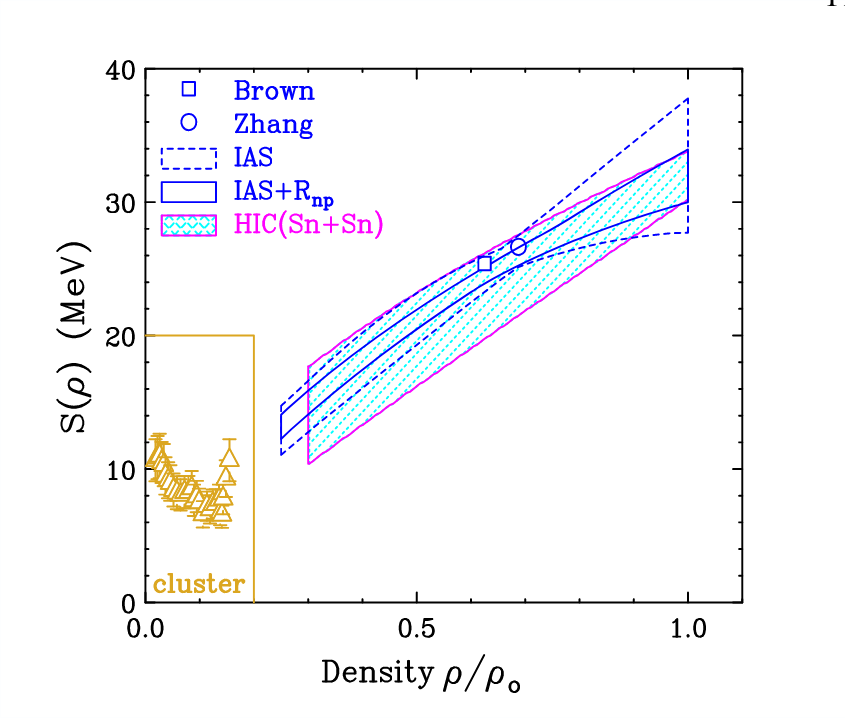
\includegraphics[scale=.5]{constraints}
\caption{Experimental constraints of the density dependence of the symmetry energy taken from \cite{awayforward}}
\label{fig:symDen}
\end{figure}


\section{Pion Observable}
\label{sec:pionObs}
It is preferable to find an observable that is easier to measure experimentally than neutrons, and is more sensitive to the just the high density region. Pions are produced though an intermediate step via $ NN \leftrightarrow \Delta$, where nucleon-nucleon collisions form an excited $\Delta$(1232) baryon resonance from one of the nucleons, which then decay decay shortly after into a pion $\Delta \leftrightarrow \pi N$. The threshold for $\Delta$ resonance production, with a mass of \SI{1232}{\mega\electronvolt\per\clight\squared}, corresponds to a laboratory beam of \SI{290}{\MeVA} in a fixed target experiment. In large nuclei, the internal motion of the nucleons is substantial and non-negligible. In the Fermi gas model, nucleons are arranged filling up higher energy levels up until they reach the Fermi energy. This extra energy allows for $\Delta$ production even at sub-threshold beam energies \cite{fermiEnergy}.


It has been shown that most of the $\Delta$'s are produced in the early dense regions of the collision \cite{mingzhang}. Figure~\ref{fig:deltaProduction} shows the average local density (c) which $\Delta$'s are produced and the number in the system (b), as a function of time in the simulation of Au + Au collisions at \SI{400}{\MeVA}. Panel (a) shows the density distribution of the density at the moment of creation for $\Delta$'s. Since the average lifetime of the $\Delta$  is $\tau_{\Delta} = \SI{1.7}{\femto\metre\per\clight}$, the $\Delta$ resonance has very little time to be affected by the medium before decaying into a $\pi$ and nucleon. Thus the outgoing $\pi$ contains information on the high density region of the collision. 

\begin{figure}[!htb]
\centering
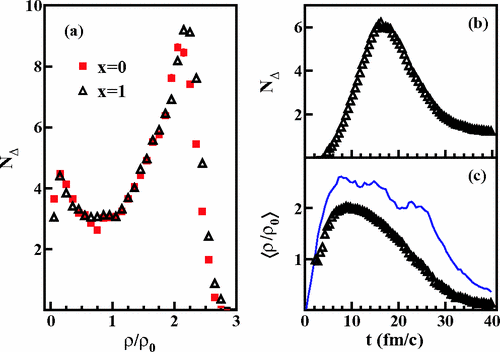
\includegraphics[width=.6\textwidth]{deltaProduction.png}
\caption{Figure taken from \cite{mingzhang} for Au + Au collisions at \SI{400}{\MeVA}. Panel (a) shows the density in the region of the $\Delta$ resonance creation for two different symmetry energies (x=0 soft) and (x=1 stiff). Panel (b) and (c) show the evolution of collision in time steps, where (b) shows the number of deltas in the system as a function of time and (c) shows the mean local baryon density in the region where $\Delta$ resonances are produced. The blue line in (c) represents the average baryon density in the most central region of the collision. This evidence shows that a majority of $\Delta$'s are produced in the high density region of the early collision.}
\label{fig:deltaProduction}
\end{figure}

The branching ratio of the various flavors of $\Delta$'s are given by the Clebsh-Gordon coefficients as shown in \ref{appen:deltadecay}. Here we see that in general p-p collisions give rise primarily to  $\pi^+$ and n-n collisions give rise to primarily $\pi^-$. In this $\Delta$ resonance model the charged pion ratio can be described as,

\begin{equation}
\frac{\pi^-}{\pi^+} = \frac{ 5N^2 + ZN }{5Z^2 + ZN}.
\label{eq:deltaModel}
\end{equation}

In this $\Delta$ resonance model, $\pi^-/\pi^+ \approx (N/Z)^2$ where $N/Z$ is the neutron-proton ratio of the dense central collision where they are produced. Pions can be reabsorbed into a $\Delta$ resonance after colliding with another nucleon in the backward process of $\Delta \leftrightarrow \pi N$. This process generally dilutes the pion sensitivity to the high density region, since with each absorption and re-emission changes the pion dynamics or even the charge of the pion reflecting the neutron-proton asymmetry at the point of creation and re-emission. Total pion absorption, back into two nucleons, requires a three body process; the pion collides with a nucleon creating a $\Delta$ resonance, then another nucleon must quickly collide with the resonance to create two nucleons. Since this is a three body process,h total pion absorption (removing them from the system) is a smaller effect than the absorption and re-emission process. Aside from these two effects which degrade the observable, in general the $\pi^-$ and $\pi^+$ are connected with n-n and p-p behavior in the high density, early collision; effectively turning the neutron measurement into a charged $\pi^-$ measurement, which is much easier to measure experimentally, and probing the high density region more than any other observable. 

\section{Motivation for Thesis}
In an effort to answer the high density behavior of the symmetry energy, we designed a new detector and a set of experiments of Sn + Sn collisions at \SI{270}{\MeVA}. Here we utilized inverse kinematics where the beam is made of a radio-active neutron rich beam impinging on a stable Sn target. We can probe the isospin asymmetry of the symmetry energy by changing the neutron-proton asymmetry of the incoming beam. Pion production has been studied before in stable beams for beam energies of \SI{400}{\MeVA} and above \cite{fopi}. Yet in these previous experiments, only total pion yields were published and no pion spectra was not published. It was also known that the efficiency analysis of the FOPI detector was particularly difficult especially for low energy pions. Although the pion production increases with the beam energy, the effects of the symmetry energy decrease. This is because higher beam velocities mean the time two nuclei spend together becomes shorter, shortening the time in which the symmetry energy can affect nucleons.  The goal of this Thesis was to design and build a high efficiency detector in order to measure pion and light charged particle spectra resulting from HICs. To do this a new Time Projection Chamber (TPC) was made called the SAMURAI pion Reconstruction Ion Tracker (\spirit) Time Projection Chamber (TPC).

%nuclear chart
%Dense nuclear matter 
%Liquid drop model explain density around saturation
%explain symmetry energy 
%extend to systems of larger pressure, isospin assymetry 
%symmetry energy how to calculate 
%Previous constraints on symmetry energy
%heavy ion collisions only way to probe density and 
%dynamics of proton neutrons 

%pion production 



\begin{comment}

\section{From Nuclear Forces to the Equation of State}
Isospin as a good quantum number at low energies 
Figure showing the nuclear forces for the pp, pn, nn 
Pauli exclusion 
inter particle distance , saturation density (maybe figure of all densities?)
Building the infinite matter
Statistical model 
Forces manifest in Energy/particle 

\section{The Nuclear Equation of State}
Figure showing the binding energy vs p-n asym
Liquid drop model, mass equation, move to higher densities
Symmetric EoS asymmetric EoS(symmetry energy)
Density dependence of the symmetry energy 

\section{Phases of Nuclear Matter}
gas liquid phase, gas, where are we
Progression through the heavy ion collision 
liquid, liquid gas, gas 

\section{Studying EoS through Heavy Ion Collisions}
going from infinite matter to finite matter 
approximate nuclear matter with neutron rich radioactive ion beams
probe different asymmetries 
probe different densities with different beam energies 
Symmetry energy goes down at higher beam energies

\section{Boltzmann Ulong Uhlenbeck (BUU) Transport Code}
Does not reach equilibrium for all observable (hadrons) what about pions?
Build up a mean field picture (momentum dependent) unknown quantities here
Non equilibrium can be solved with Boltzman equation with collision term and solved by MC
Figure of transport simulation code showing collision progression 
Clustering is an issue 
Meson, resonance production 

\section{Observables of interest to the EoS}
Particle yields of isospin opposites 
Flow??
Figure showing p-n observable lessens at high energy and from all densities 

\section{Pion Production }
Figure showing delta resonance 
Figure showing pion's produced at 2po 
Figure showing fermi motion effect (not really sub threshold but ok)
(chemical potential model, delta isobar) prediction for pion ratio
pion mass is small momentum shifted by coulomb affecting shape of pion spectra

\section{Previous Constraints}
Figure showing GW constraint and other previous constraints 
FOPI data at 400 A MeV not as sensitive to symmetry energy 
Saturation density and lower constrained but issues at high density
conflicting analysis on FOPI data which was not intended to be used for Symm Energy
Can you group all the constraints to one nice plot???

\section{Motivation for building the S$\pi$RIT TPC}
Based on EOS TPC
High efficiency for detecting pions and other light charged particles 
Effort to reduce the experimental error bars on such spectra which theory could use


\end{comment}